\section{Vypracování}
\subsection{Digitální model terénu a polyedrický model}

Základní úlohou při analýze výškopisu v geografických informačních systémech je vytvoření digitálního modelu terénu (DMT). V této práci je terén reprezentován pomocí nepravidelné trojúhelníkové sítě (TIN – Triangulated Irregular Network). 
Pro vytvoření základní sítě hran nad množinou 3D bodů $P = \{p_1, \dots, p_n\}$ byla implementována Delaunayho triangulace. 

Aby bylo možné nad modelem provádět analytické úlohy, je nutné síť hran převést na plnohodnotný polyedrický model. Plošky jsou představovány trojúhelníky se společnou hranou. Proložením rovin třemi vrcholy každého trojúhelníku v prostoru ${R}^3$ vznikne nepravidelný mnohostěn, který se přimyká k terénu. Parametry těchto rovin jsou nezbytné pro následné výpočty sklonu a expozice.

\subsection{Konstrukce vrstevnic}

Vrstevnice jsou izolinie spojující body se stejnou nadmořskou výškou. V polyedrickém modelu jsou generovány pomocí lineární interpolace na hranách jednotlivých trojúhelníků. Algoritmus postupně protíná trojúhelníkovou síť vodorovnými rovinami s definovaným krokem $\Delta z$. 

U každého trojúhelníku se vyhodnocují výškové rozdíly jeho vrcholů vůči testované rovině $z$. Pokud rovina protíná dvě hrany trojúhelníku, vypočítají se souřadnice průsečíků a tyto dva body vytvoří úsečku vrstevnice. 
\\[2mm]

\textbf{Použitý kód výpočtu průsečíku}

\begin{lstlisting}[language=Python, caption = Implementace lineární interpolace pro nalezení bodu vrstevnice.]
    def getContourPoint(self, p1, p2, z):
        #Compute intersection line and plane
        xb = (p2.x() - p1.x())/(p2.z() - p1.z()) * (z - p1.z()) + p1.x()
        yb = (p2.y() - p1.y())/(p2.z() - p1.z()) * (z - p1.z()) + p1.y()
        
        return QPoint3DF(xb, yb, z)
\end{lstlisting}


\subsection{Analýza sklonu terénu}

Analýza sklonu je analytická úloha realizovaná nad DMT, jejíž zprostředkující hodnotou je gradient (vektor maximálního spádu). Rovina $\rho$ procházející třemi body trojúhelníku je definována normálovým vektorem $\vec{n} = (a, b, c)$. V aplikaci je tento vektor získán vektorovým součinem dvou směrových vektorů tvořících hrany trojúhelníku.

Odchylka $\varphi$ (sklon) roviny trojúhelníku od vodorovné roviny je následně vypočtena pomocí arkus kosinu podílu vertikální složky $c$ a celkové velikosti normálového vektoru:
$$ \varphi = \arccos\left(\frac{|c|}{\sqrt{a^2 + b^2 + c^2}}\right) $$
Pro vizualizaci jsou trojúhelníky dynamicky vybarvovány barevnou škálou (od zelené po červenou) na základě poměru jejich sklonu k maximálnímu detekovanému sklonu v daném modelu.
\\[2mm]

\begin{figure}
    \centering
    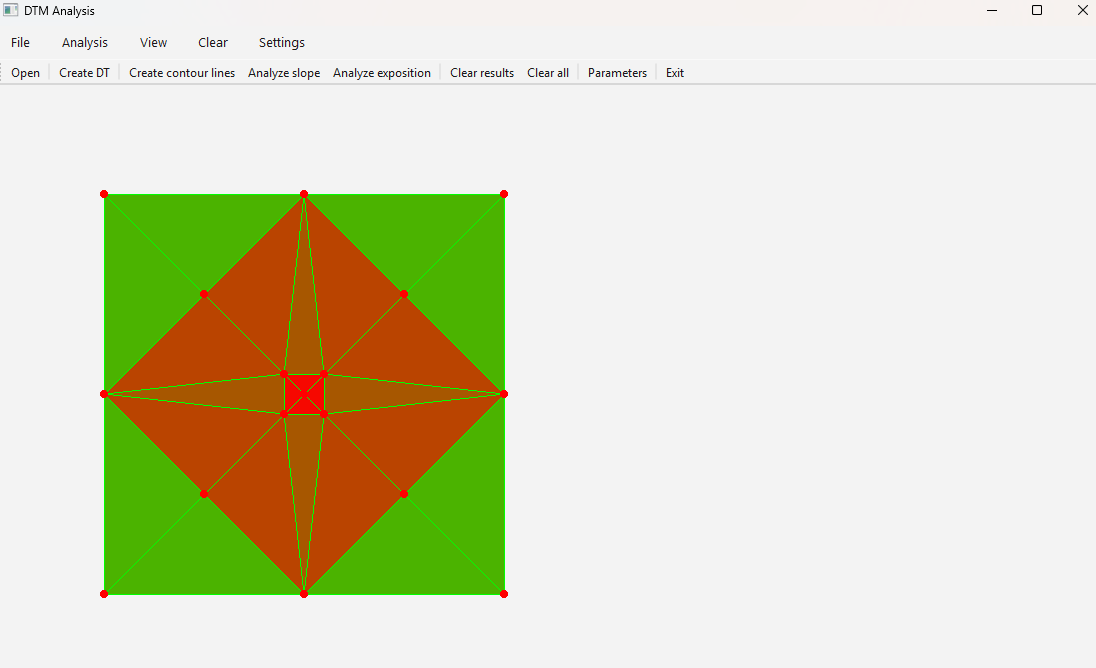
\includegraphics[width=0.9\linewidth]{figures/Slope.png}
    \caption{Printscreen vytvořené aplikace s výpočtem sklonu.}
    \label{fig:obr1}
\end{figure}

\subsection{Analýza expozice terénu}

Expozice (orientace) terénu je definována jako azimut průmětu gradientu do vodorovné roviny $xy$. Využívá se zde stejný normálový vektor $\vec{n} = (a, b, c)$ jako při výpočtu sklonu, pro orientaci se ale využívají pouze složky $a$ a $b$. 

Azimut $A$ je měřen od osy $y$. Pro správnou detekci kvadrantů a předcházení chybám při dělení nulou je místo klasického arkus tangens využita funkce \texttt{atan2}. Výsledný úhel je normalizován do intervalu $\langle 0^\circ, 360^\circ \rangle$. Pro vizualizaci je použit barevný model HSL (Hue, Saturation, Lightness), který umožňuje plynulý kruhový přechod barev přes všechny světové strany.
\\[2mm]

\begin{figure}
    \centering
    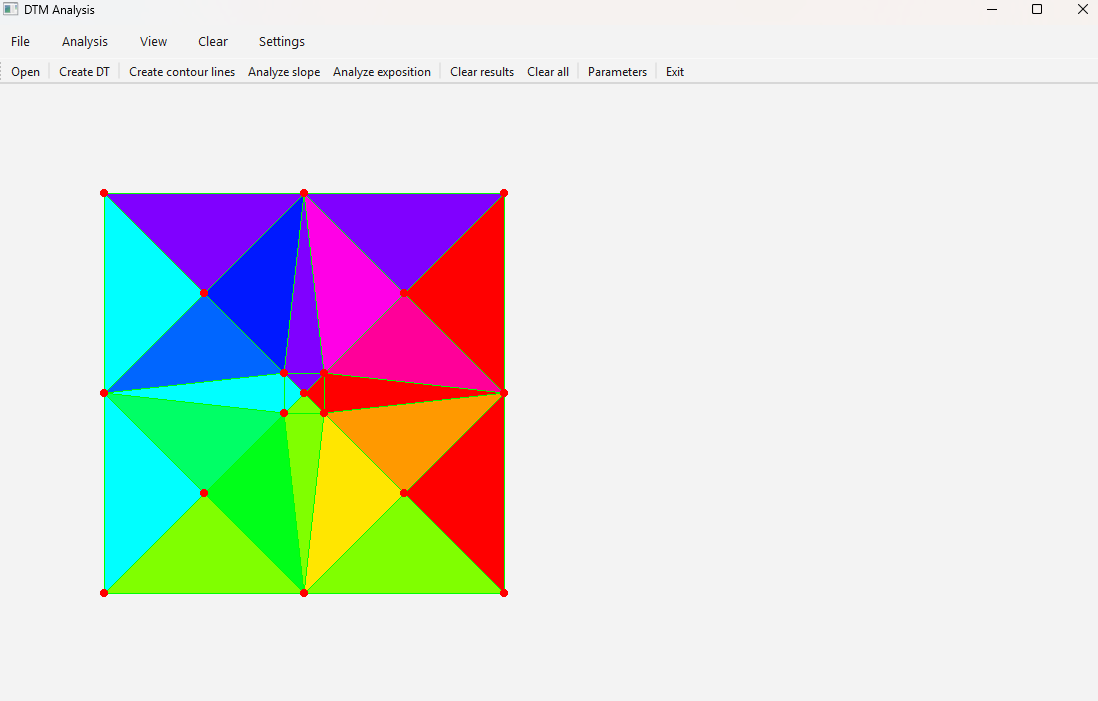
\includegraphics[width=0.9\linewidth]{figures/Expostiton.png}
    \caption{Printscreen vytvořené aplikace se znázorněným výpočtem expozice.}
    \label{fig:obr1}
\end{figure}



\subsection{Načtení vstupních dat}
Vstupními daty jsou textové soubory obsahující prostorové souřadnice bodů. Každý řádek souboru reprezentuje jeden bod ve formátu X, Y a Z, oddělených mezerou. Načítání je řešeno pomocí standardního dialogového okna, po kterém se soubor iterativně zpracovává po řádcích, data se převádí na desetinná čísla a transformují se do objektů \texttt{QPoint3DF}.
\begin{lstlisting}[language=Python, caption = Použití souřadnic z textového souboru.]
    with open(file_path, 'r') as file:
                for line in file:
                    #Split line into coordinates and convert to float
                    coords = line.strip().split()
                    if len(coords) == 3:
                        x = float(coords[0])
                        y = float(coords[1])
                        z = float(coords[2])
                        points.append(QPoint3DF(x, y, z))
\end{lstlisting}


\subsection{Dokumentace}
\subsubsection{Třída Algorithms}
Třída Algorithms zahrnuje veškeré matematické a výpočetní metody. Obsahuje funkce pro konstrukci Delaunayho triangulace, generování izolinií (vrstevnic), sestavení polyedrického modelu (TIN) a metody analyzeSlope a analyzeExposition realizující výpočet terénních charakteristik z normálových vektorů.

\subsubsection{Třída Draw}
Třída Draw rozšiřuje widget kreslícího plátna a obsahuje metody pro grafickou reprezentaci dat. Stará se o vykreslování bodů, vrstevnic a sítě trojúhelníků. Uchovává stav vykreslovacího módu (\texttt{\_\_draw\_mode}) a na jeho základě dynamicky obarvuje polygony TINu buď lineární interpolací červené a zelené barvy (pro sklon), nebo pomocí HSL palety (pro expozici).

\subsubsection{Třída Main Form}
Třída MainForm slouží ke spuštění grafického uživatelského rozhraní aplikace, spravuje nástrojové lišty (ToolBar) a propojuje uživatelské akce (tlačítka) s výkonnými metodami definovanými ve třídách Algorithms a Draw. Zajišťuje rovněž bezpečné otevírání souborů a chybová hlášení.

\subsection{Závěr}
V rámci této práce byla úspěšně vytvořena aplikace v prostředí PyQt6, která řeší tvorbu a analýzu digitálního modelu terénu. Byla naimplementována plně funkční Delaunayho triangulace, sestavení polyedrického TIN modelu a generování vrstevnic s dynamickým výpočtem výškového rozmezí. Aplikace bezpečně řeší výpočty sklonu i expozice s využitím vektorové matematiky a ošetřením chyb plovoucí desetinné čárky.

Správnost a stabilita algoritmů, stejně jako vizuální plynulost barevných palet, byla mimo jiné úspěšně ověřena na reálných výškových profilech povrchových útvarů z vesmírných misí (např. kráter Nightingale na planetce Bennu z mise OSIRIS-REx nebo útes Hathor na kometě 67P ze sondy Rosetta).







